% Method figure for the README. Build: powershell -File build.ps1  ->  ../method.png (+ method.pdf)
% The robot always stands for the model (gpt-6-luna); code steps get plain icons.
\documentclass[tikz,border=4pt]{standalone}
\usepackage[T1]{fontenc}
\usepackage{times}
\usepackage[scaled=0.92]{helvet}
\renewcommand{\ttdefault}{lmtt}
\usepackage{amssymb,pifont}
\usepackage{tikz}
\usetikzlibrary{arrows.meta,calc,shapes.callouts}

% ------------------------------------------------------------------ palette
\definecolor{cData}{HTML}{4F6FA8}   % records, questions
\definecolor{cLLM}{HTML}{7555A3}    % model steps
\definecolor{cCode}{HTML}{1F8A7C}   % code steps
\definecolor{cStore}{HTML}{A8781B}  % saved abstraction
\definecolor{cGood}{HTML}{3D8A4A}
\definecolor{cBad}{HTML}{C44536}
\definecolor{cWarn}{HTML}{B7791F}
\definecolor{ink}{HTML}{23262B}
\definecolor{mute}{HTML}{646A75}
\definecolor{rule}{HTML}{C9CDD4}
\definecolor{hl}{HTML}{FFE58A}

\newcommand{\hv}{\fontfamily{phv}\selectfont}
\newcommand{\fs}[1]{\fontsize{#1}{#1}\selectfont}
\newcommand{\ok}{\ding{51}}
\newcommand{\no}{\ding{55}}
\tikzset{
  every node/.style={font=\hv\fs{5.6}, text=ink, inner sep=1pt},
  stage/.style={rounded corners=5pt, draw=#1!75, fill=#1!7, line width=0.8pt},
  title/.style={font=\hv\bfseries\fs{8}, text=#1!85!black},
  capt/.style={font=\hv\fs{5.1}, text=mute, align=center},
  lab/.style={font=\hv\bfseries\fs{5.6}, text=#1},
  mono/.style={font=\ttfamily\fs{4.5}},
  arr/.style={-{Latex[length=5pt,width=4.5pt]}, line width=1.3pt, draw=ink},
  arrc/.style={-{Latex[length=5pt,width=4.5pt]}, line width=1.3pt, draw=#1},
  thin/.style={-{Latex[length=3.4pt,width=3.2pt]}, line width=0.8pt, draw=#1},
  flow/.style={rounded corners=2pt, draw=#1, fill=#1!9, text=#1!70!black,
               font=\hv\bfseries\fs{5.3}, minimum height=0.5cm, text width=2.0cm,
               align=center, inner sep=1pt, line width=0.6pt},
  farr/.style={-{Latex[length=3.2pt,width=3pt]}, line width=0.8pt, draw=#1},
  tool/.style={rounded corners=1.2pt, draw=cCode!80, fill=white, text=cCode!75!black,
               font=\ttfamily\bfseries\fs{4.4}, minimum height=0.25cm, minimum width=1.85cm, inner sep=0.8pt},
  sq/.style={rounded corners=0.6pt, fill=#1, minimum size=0.13cm, inner sep=0pt},
}

% ------------------------------------------------------------------ icons (x, y, scale, colour)
\newcommand{\doci}[4]{\begin{scope}[shift={(#1,#2)}, scale=#3]
    \filldraw[fill=white, draw=#4, line width=0.5pt] (-0.09,-0.12) -- (-0.09,0.12) -- (0.04,0.12) -- (0.09,0.07) -- (0.09,-0.12) -- cycle;
    \draw[#4, line width=0.3pt] (0.04,0.12) -- (0.04,0.07) -- (0.09,0.07);
    \foreach \y in {0.05,0.01,-0.03,-0.07} \draw[#4!80, line width=0.35pt] (-0.06,\y) -- (0.06,\y);\end{scope}}
\newcommand{\geari}[3]{\begin{scope}[shift={(#1,#2)}, scale=#3]
    \fill[cCode] (0,0) circle (0.1);
    \foreach \a in {0,45,...,315} \fill[cCode, rotate=\a] (-0.028,0.08) rectangle (0.028,0.135);
    \fill[cCode!7] (0,0) circle (0.042);\end{scope}}
\newcommand{\dbi}[3]{\begin{scope}[shift={(#1,#2)}, scale=#3]
    \filldraw[fill=cStore!15, draw=cStore, line width=0.5pt] (-0.1,0.08) -- (-0.1,-0.08) arc (180:360:0.1 and 0.035) -- (0.1,0.08);
    \draw[cStore, line width=0.5pt] (-0.1,0.0) arc (180:360:0.1 and 0.035);
    \filldraw[fill=cStore!35, draw=cStore, line width=0.5pt] (0,0.08) ellipse (0.1 and 0.035);\end{scope}}

\begin{document}
\begin{tikzpicture}[x=1cm, y=1cm]
\path[use as bounding box] (0,0) rectangle (13.97,6.38);

% section header + legend
\node[anchor=west, font=\hv\bfseries\fs{6.8}] at (0.05,6.22) {1\quad Build the abstraction};
\node[anchor=west, font=\hv\itshape\fs{5.3}, text=mute] at (2.95,6.21) {once per new document; results are cached};
\node[anchor=east, inner sep=0] at (13.92,6.22) {%
  \tikz[baseline=-0.6ex]\node[sq=cLLM]{};\ \textcolor{cLLM!80!black}{\bfseries model}\quad
  \tikz[baseline=-0.6ex]\node[sq=cCode]{};\ \textcolor{cCode!80!black}{\bfseries code}\quad
  \tikz[baseline=-0.6ex]\node[sq=cStore]{};\ \textcolor{cStore!80!black}{\bfseries saved data}\quad
  \tikz[baseline=-0.6ex]\node[sq=cData]{};\ \textcolor{cData!80!black}{\bfseries input}};

\def\yb{3.85} \def\yt{6.02} \def\yT{5.8} \def\ya{4.95}

% ================================================================== top row
% ---- Records
\draw[stage=cData] (0.05,\yb) rectangle (1.7,\yt);
\node[title=cData] at (0.875,\yT) {Records};
\doci{0.55}{5.08}{2.3}{cData} \doci{0.875}{4.98}{2.3}{cData} \doci{1.2}{4.88}{2.3}{cData}
\node[lab=ink] at (0.875,4.4) {31 documents};
\node[capt] at (0.875,4.09) {notes, rosters,\\[-1pt]corrections, copies};

% ---- Ingest
\draw[stage=cCode] (2.0,\yb) rectangle (3.45,\yt);
\node[title=cCode] at (2.725,\yT) {Ingest};
\doci{2.43}{5.16}{1.9}{cCode} \doci{3.02}{5.16}{1.9}{cCode}
\node[font=\hv\bfseries\fs{9}, text=cCode] at (2.725,5.16) {=};
\node[draw=cCode!80, fill=white, rounded corners=1.2pt, font=\ttfamily\bfseries\fs{4.8}, text=cCode!75!black, inner sep=1.5pt] at (2.725,4.62) {sha-256};
\node[capt] at (2.725,4.09) {duplicates never\\[-1pt]reach the model};

% ---- Extract (model)
\draw[stage=cLLM] (3.75,\yb) rectangle (6.55,\yt);
\node[title=cLLM] at (5.15,\yT) {Extract};
\node[inner sep=0] at (4.24,4.95) {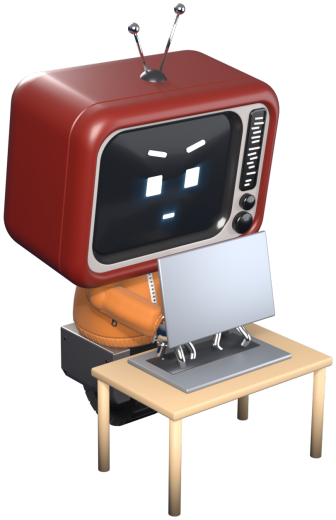
\includegraphics[height=1.15cm]{img/robot_build.png}};
\node[anchor=west, draw=cLLM!60, fill=white, rounded corners=1.5pt, inner sep=2pt, align=left, mono, text=cLLM!75!black] at (4.66,4.95)
  {date\ \ 2026-01-21\\[-0.5pt]type\ \ individual\\[-0.5pt]times 13:00--13:20\\[-0.5pt]\ \ \ \ \ \ 13:30--13:55\\[-0.5pt]quote ``Patient contact\\[-0.5pt]\ \ \ \ \ \ occurred ...''};
\node[capt] at (5.15,4.09) {one call per document;\\[-1pt]times as written, no totals};

% ---- Verify quotes (code)
\draw[stage=cCode] (6.85,\yb) rectangle (8.25,\yt);
\node[title=cCode] at (7.55,\yT) {Verify};
\begin{scope}[shift={(7.43,5.05)}]
  \filldraw[fill=white, draw=cCode, line width=0.6pt] (-0.25,-0.32) -- (-0.25,0.32) -- (0.14,0.32) -- (0.25,0.21) -- (0.25,-0.32) -- cycle;
  \foreach \y in {0.18,0.08,-0.12,-0.22} \draw[cCode!70, line width=0.5pt] (-0.17,\y) -- (0.17,\y);
  \fill[hl] (-0.2,-0.06) rectangle (0.2,0.04); \draw[cCode!70, line width=0.5pt] (-0.17,-0.01) -- (0.17,-0.01);
  \draw[cCode!80!black, line width=1.6pt] (0.31,-0.2) -- (0.45,-0.36);
  \filldraw[fill=white, fill opacity=0.35, draw=cCode!80!black, line width=1.1pt] (0.2,-0.08) circle (0.15);
\end{scope}
\node[font=\hv\bfseries\fs{7.4}, text=cCode!80!black] at (7.55,4.42) {137 / 137};
\node[capt] at (7.55,4.09) {quotes found in\\[-1pt]their source};

% ---- Reconcile (code)
\draw[stage=cCode] (8.55,\yb) rectangle (11.0,\yt);
\node[title=cCode] at (9.9,\yT) {Reconcile};
\geari{8.9}{\yT}{1.0}
\node[anchor=north west, inner sep=0, align=left, font=\hv\fs{4.9}] at (8.68,5.54) {%
  \setlength{\tabcolsep}{1.6pt}\renewcommand{\arraystretch}{1.05}%
  \begin{tabular}{@{}cl@{}}
  \textcolor{cCode}{\bfseries 1} & One encounter, one contact\\
  \textcolor{cCode}{\bfseries 2} & Signed beats copy, draft, bill\\
  \textcolor{cCode}{\bfseries 3} & Only corrections override\\
  \textcolor{cCode}{\bfseries 4} & Minutes = present $-$ breaks\\
  \textcolor{cCode}{\bfseries 5} & Conflict $\to$ range + issue
  \end{tabular}};
\node[capt] at (9.775,4.09) {rules in code: the same\\[-1pt]result on every run};

% ---- Abstraction (saved data)
\draw[stage=cStore] (11.3,\yb) rectangle (13.92,\yt);
\node[title=cStore] at (12.75,\yT) {Abstraction};
\dbi{11.68}{\yT-0.03}{1.25}
\node[anchor=north, inner sep=0, font=\hv\fs{4.9}] at (12.64,5.55) {%
  \setlength{\tabcolsep}{1.9pt}\renewcommand{\arraystretch}{1.1}%
  \begin{tabular}{@{}lrl@{}}
  Jan 19 group  & 60 min  & \textcolor{cGood}{\ok}\\
  Jan 21 video  & 45 min  & \textcolor{cGood}{\ok}\\
  Jan 26 indiv. & 40--50  & \textcolor{cWarn}{\bfseries ! range}\\
  Jan 27 group  & 0 min   & \textcolor{cBad}{\no\ no-show}
  \end{tabular}};
\node[capt] at (12.61,4.09) {SQLite: every contact, issue and\\[-1pt]number links to its quote};

% ---- top flow
\draw[arr] (1.7,\ya) -- (2.0,\ya);
\draw[arr] (3.45,\ya) -- (3.75,\ya);
\draw[arr] (6.55,\ya) -- (6.85,\ya);
\draw[arr] (8.25,\ya) -- (8.55,\ya);
\draw[arr] (11.0,\ya) -- (11.3,\ya);

% ================================================================== bottom row
\node[anchor=west, font=\hv\bfseries\fs{6.8}] at (0.05,3.42) {2\quad Answer a question};
\node[anchor=west, font=\hv\itshape\fs{5.3}, text=mute] at (2.45,3.41) {nothing is re-extracted};
\def\bb{0.42} \def\bt{2.97} \def\bT{2.75}

% abstraction feeds the queries
\draw[arrc=cStore] (12.61,\yb) -- (12.61,3.66) -- (5.475,3.66) -- (5.475,\bt);
\node[lab=cStore, fill=white, inner sep=1.2pt] at (9.0,3.66) {queries read the saved abstraction};

% ---- Question
\draw[stage=cData] (0.05,\bb) rectangle (1.75,\bt);
\node[title=cData] at (0.9,\bT) {Question};
\node[rectangle callout, callout relative pointer={(-0.12,-0.22)}, rounded corners=3pt, draw=cData, fill=white,
      line width=0.6pt, text width=1.3cm, align=center, font=\hv\fs{5.3}, inner sep=3pt] at (0.9,1.85)
  {How many minutes did Rowan get each week?};
\node[capt] at (0.9,0.75) {any new question;\\[-1pt]no rebuild needed};

% ---- Model (plans, then writes)
\draw[stage=cLLM] (2.05,\bb) rectangle (3.85,\bt);
\node[title=cLLM] at (2.95,\bT) {Model};
\node[inner sep=0] at (2.95,1.83) {
\includegraphics[height=1.25cm]{img/robot_think.png}};
\node[capt] at (2.95,0.75) {picks queries, then\\[-1pt]writes; does no sums};

% ---- Queries (code)
\draw[stage=cCode] (4.4,1.0) rectangle (6.55,\bt);
\node[title=cCode] at (5.475,\bT) {Queries};
\foreach \t [count=\i] in {weekly\_summary, goal\_compliance, day\_detail, measures, get\_document\_passage}
  \node[tool] at (5.475,2.62-0.235*\i) {\t()};
\node[capt] at (5.475,1.17) {all numbers come from here};

% model <-> queries
\draw[thin=cLLM] (3.85,2.15) -- (4.4,2.15);
\draw[thin=cCode] (4.4,1.7) -- (3.85,1.7);
\node[font=\hv\fs{4.4}, text=cLLM!80!black] at (4.125,2.27) {call};
\node[font=\hv\fs{4.4}, text=cCode!80!black] at (4.125,1.82) {result};

% draft answer -> quote check, under the Queries box
\draw[arrc=cLLM] (3.85,0.68) -- (6.85,0.68);
\node[lab=cLLM, fill=white, inner sep=1pt] at (5.475,0.68) {draft answer};

% ---- Quote check (code)
\draw[stage=cCode] (6.85,\bb) rectangle (8.65,\bt);
\node[title=cCode] at (7.75,\bT) {Quote check};
\node[font=\rmfamily\bfseries\fs{26}, text=cCode, inner sep=0] at (7.75,1.85) {``\,''};
\node[capt] at (7.75,1.0) {each quote must be in\\[-1pt]the document it cites};

% ---- outcome: verified
\draw[arrc=cGood] (8.65,2.1) -- (9.15,2.1);
\node[inner sep=0] at (9.62,2.1) {
\includegraphics[height=1.05cm]{img/robot_cheer.png}};
\draw[rounded corners=4pt, draw=cGood!70, fill=white, line width=0.8pt] (10.15,1.47) rectangle (13.92,2.97);
\node[anchor=north west, align=left, text width=3.55cm, font=\hv\fs{5.3}, inner sep=0] at (10.26,2.86) {%
  \textbf{\textcolor{cGood!85!black}{All quotes found: answer shown}}\\[2pt]
  \raggedright Weeks 1--2 not met, week 3 met, week 4 undetermined (Jan 26 is 40--50 min) \mbox{\textcolor{cData}{\bfseries [BH-D003] [BH-D110]}}};
\node[anchor=south east, font=\hv\bfseries\fs{4.8}, text=cGood!85!black, fill=cGood!12, rounded corners=1.5pt, inner sep=1.5pt]
  at (13.85,1.55) {\ok\ 5/5 quotes verified};

% ---- outcome: a quote is missing
\draw[arrc=cBad] (8.65,0.95) -- (9.15,0.95);
\node[inner sep=0] at (9.64,0.95) {
\includegraphics[height=0.95cm]{img/robot_fix.png}};
\node[lab=cBad, anchor=west, align=left] at (10.17,1.08) {Quote not found: one repair pass};
\node[capt, anchor=west, align=left] at (10.17,0.78) {then checked again; anything still\\[-1pt]missing is shown with the answer};
\draw[cBad, line width=0.8pt, dash pattern=on 2.4pt off 1.6pt, -{Latex[length=3.4pt,width=3.2pt]}]
  (9.64,0.47) -- (9.64,0.2) -- (2.95,0.2) -- (2.95,\bb);
\end{tikzpicture}
\end{document}
